\section{Introduction}
This work is submitted in partial fulfilment of the course CS120: Computer network at ShanghaiTech University. The network stack is an essential topic in computer networks and has various implementations. To comprehensively understand it, we are asked to implement our network stack Athernet. \par
Unlike traditional wireless or wired methods, Athernet uses sound waves to transmit data between devices. The stack has implemented the basic functionalities of the standard TCP/IP and can be used with existing network infrastructure. Additionally, the system has the potential to be used in areas where wireless communication is not feasible, such as underwater communications.\par
\begin{figure}[H]
	\begin{center}
		\centerline{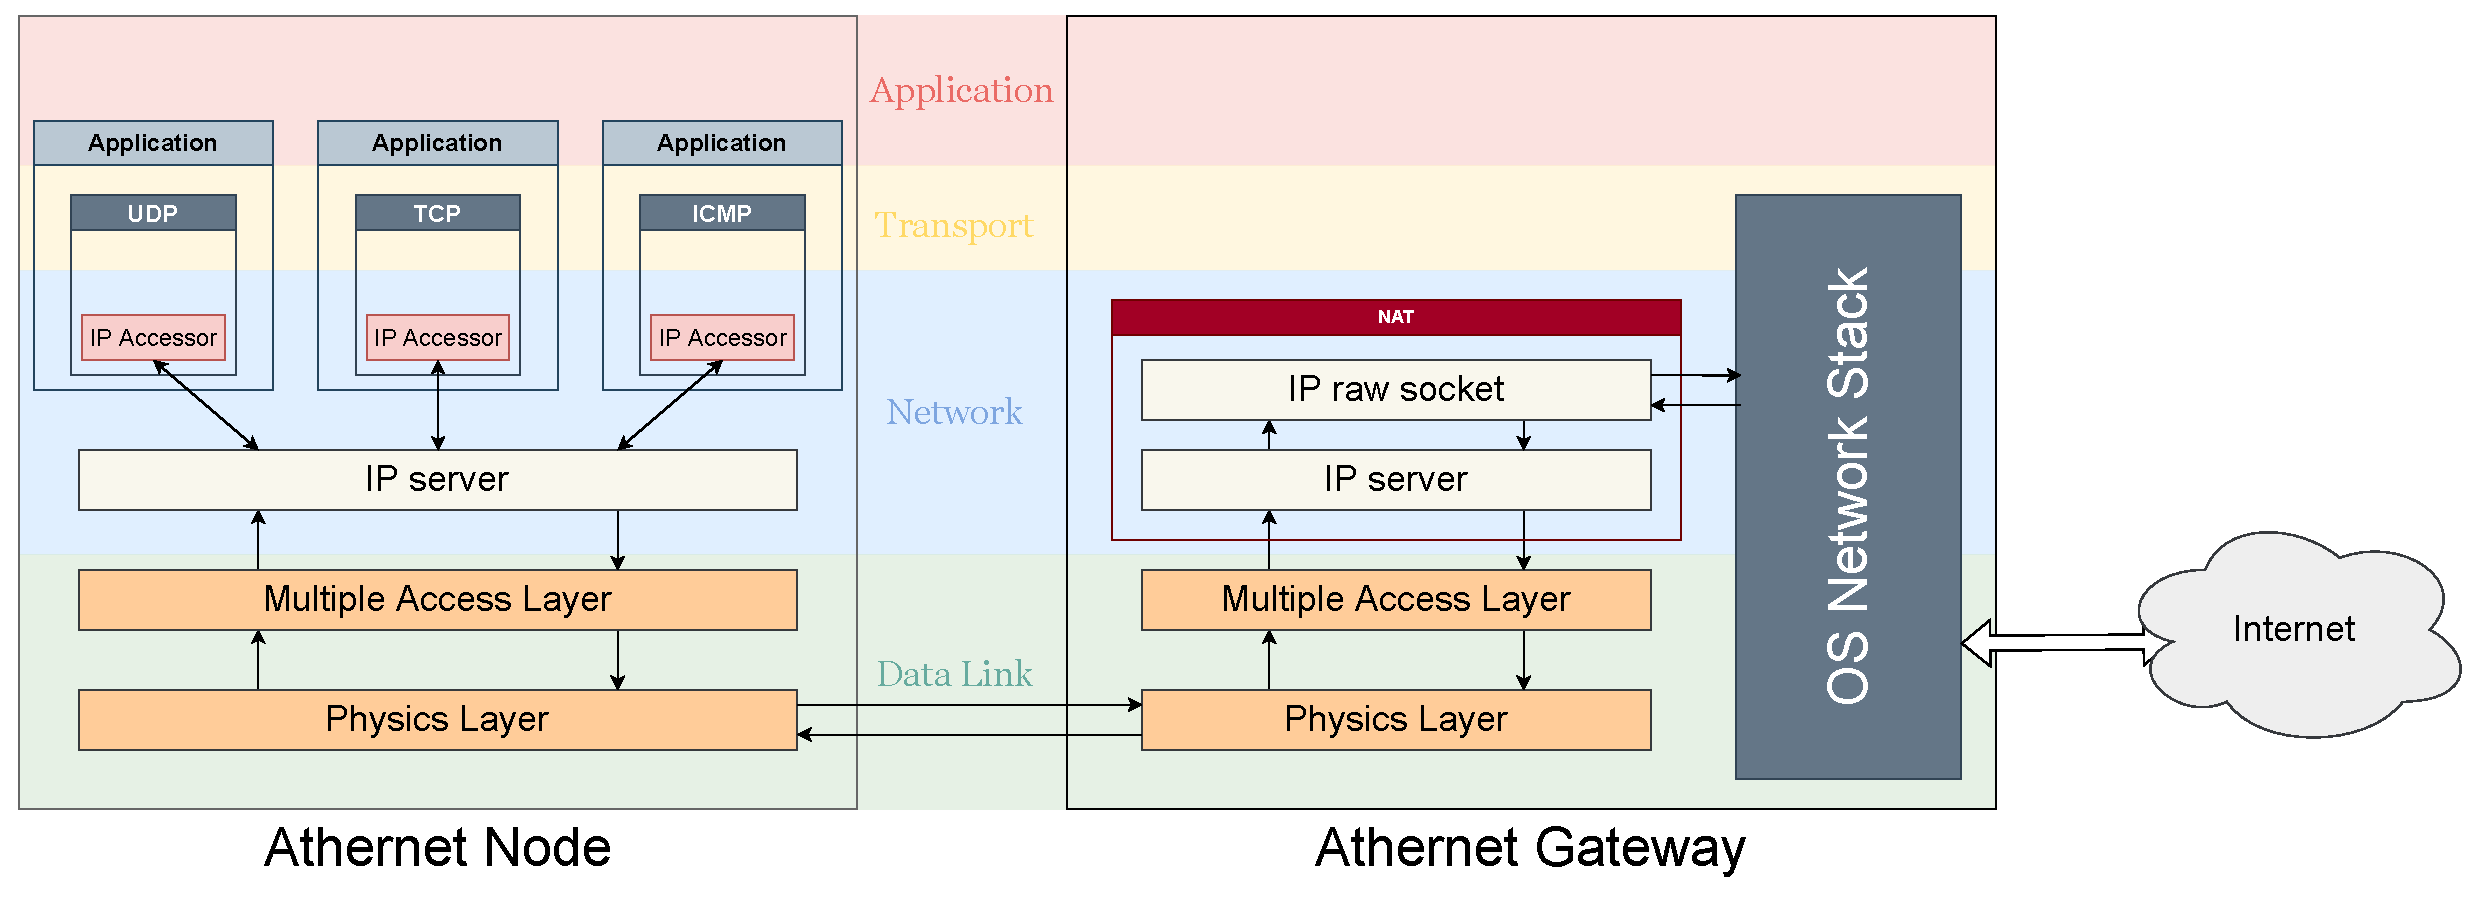
\includegraphics[width=\columnwidth]{./figures/overview.pdf}}
		\caption{the overview architecture of the Athernet network stack}
		\label{overview}
	\end{center}
\end{figure}

The network stack is composed of the following four layers where each layer is built on the previous one.
\begin{itemize}
	\item \textbf{The link layer:} The link layer provides reliable bidirectional data transmission in local area.
	      It is decomposed into two sublayers namely the \emph{physics sublayer} and the \emph{media access control sublayer}.
	      The physical layer is responsible for the converting digital data into audio signal or the reverse process and sending/receiving data through sound waves.
	      It supports both noisy wireless medium and audio cable media.
	      Two different modulation schemes are implemented for the two scenarios: a passband modulation scheme that combines \emph{BPSK} and \emph{OFDM} for the wireless scenarios
	      and a baseband modulation scheme using \emph{4B5B} with \emph{NRZI} for the cable connected scenarios.
	      The media access layer deals with collisions that may happens when multiple nodes sends signal to the media simultaneously.
	      \emph{CSMA/CA} is implemented to provide reliable data transmission.
	\item \textbf{The network layer:} \emph{Internet Protocol(IP)} is implemented for inter-network data transmission.
	      An daemon process called the \emph{IP server} regularly sends packets to peers and receives packets from peers.
	      To allow programs in the next layer to access the network layer service, \emph{IP accessor} which communicates with the \emph{IP server} using unix domain socket is created.
	      The \emph{network address translation(NAT)} is also implemented in this layer, which enables the communication between Athernet LAN and the Internet.
	\item \textbf{The transport layer:} Various transport layer protocols are implemented including \emph{transmission control protocol(TCP)}, \emph{user datagram protocol(UDP)} and \emph{internet control message protocol(ICMP)}.
	      Athernet socket, a set of APIs that resembles the socket API in rust standard library, are exposed for applications to use the transport layer services.
	\item \textbf{The application layer:}
	      A simple \emph{file transfer protocol(FTP)} client supporting a set of restricted control commands and only passive transmission mode
	      is implemented on Athernet TCP to demonstrate the capability of Athernet.
          For Athernet to support the pre-existing applications which are built on OS TCP/IP stack,
	      a SOCKS5 proxy server is implemented that redirects network traffics through Athernet.
\end{itemize}
Figure~\ref{overview} shows the overall architecture of the Athernet. The Athernet nodes are interconnected and can connect to the Internet through the Athernet gateway, which runs a NAT.\par
% We select Rust as our main programing language due to its reliability and efficiency.
The paper is devided into five parts. Through chapter two to five, we describes the design of the four layers of our network stack. In the last chapter, we analyze the problems in our design and make a technical summary.
